\documentclass[12pt]{article}
%
\usepackage{makeidx}  % allows for indexgeneration
\usepackage{pslatex}
\usepackage{graphicx}
\usepackage{float}

% \makeatletter
% \newcommand{\rmnum}[1]{\romannumeral #1}
% \newcommand{\Rmnum}[1]{\expandafter\@slowromancap\romannumeral #1@}
% \makeatother
%
\begin{document}
%
%\frontmatter          % for the preliminaries

%\mainmatter              % start of the contributions
%
\title{Sequencing the Breakpoint Regions of Genome Rearrangements}
%
%\titlerunning{CAP project}  
%\author{Yu Lin}
%\institute{}

%
\maketitle              

\section{Introduction}

Genome-scale evolutionary events include genome rearrangements, duplications and deletions. 
Genome rearrangements, which shuffle gene orders and change the gene orientations, 
includes inversions, transpositions, translocations, fusions, and fissions. 

In this paper, we focus on the breakpoint regions of genome rearrangements.
Genome rearrangements represent large-scale evolutionary events that are clearly distinct from the small-scale changes as mutations and indels.
Genome rearrangements in primates evolution have been studied at different levels of resolution, 
such as comparative chromosome banding~\cite{yunis1982origin}, 
gene mapping~\cite{turleau1983gene}, 
cross-species chromosomal painting~\cite{jauch1992reconstruction,murphy2005dynamics}, 
comparative genome hybridization painting~\cite{carbone2006}, fluorescent in situ hybridization (FISH)~\cite{wienberg2005} 
and bacterial artificial chromosome (BAC)~\cite{girirajan2009}. 
Current approaches (except BAC~\cite{girirajan2009}) 
can not offer base-pair resolution to study the exact sequences at the breakpoint regions of genome rearrangements, 
while BAC~\cite{girirajan2009} has only been applied to sequence 24 breakpoint regions between human and gibbon genomes. 

The reliable and accurate assembly of large genomes from next-gen sequencing techniques 
provides an opportunity to study breakpoint regions systematically between different genomes.
Detailed sequencing analysis of human-gibbon rearrangements revealed precise breakage positions for 60\% breakpoints (see Figure~\ref{breakpoint2}(a)), 
and new insertion sequences at 40\% breakpoint regions, most of which consisted of common repeat families (e.g. Alu and LINE) 
as well as duplicate sequences that originate from neighborhood of the breakpoints~\cite{girirajan2009} (see Figure~\ref{breakpoint2}(b)).
Studies on genomic disorders from clinical chromosomal microarray analysis ~\cite{lee2007dna,liu2011chromosome}
also revealed similar complex breakpoint regions of rearrangements, with the analysis of sequences at breakpoint junctions 
by array comparative genomic hybridization (aCHG) from clinical chromosomal microarray analysis~\cite{pinkel2005array}. 
These observations support a replication based mechanism, 
the Fork Stalling and Template Switching (FoSTeS) model~\cite{lee2007dna} (inspired by a similar mechanism proposed for amplification in E. coli \cite{slack2006mechanism}) 
and the Microhomology Mediate Break-Induced Replication (MMBIR) model~\cite{hastings2009microhomology}.
According to this mechanism, during DNA replication, 
long-distance template-switching occurs between replication forks in physical proximity (not necessary adjacent in primary sequences) through the microhomology.
Depending on whether the position and orientation of the new fork was invaded and copied, and the direction of fork progression, 
template-switching results in a duplication, deletion, inversion or translation~\cite{hastings2009microhomology}.
This procedure of long-distance template-switching could occur multiple times in series, 
due to the poor processivity of the involved DNA polymerase, causing the complex breakpoint regions of rearrangements~\cite{gu2008mechanisms}.

\begin{figure}[H]
\begin{center}
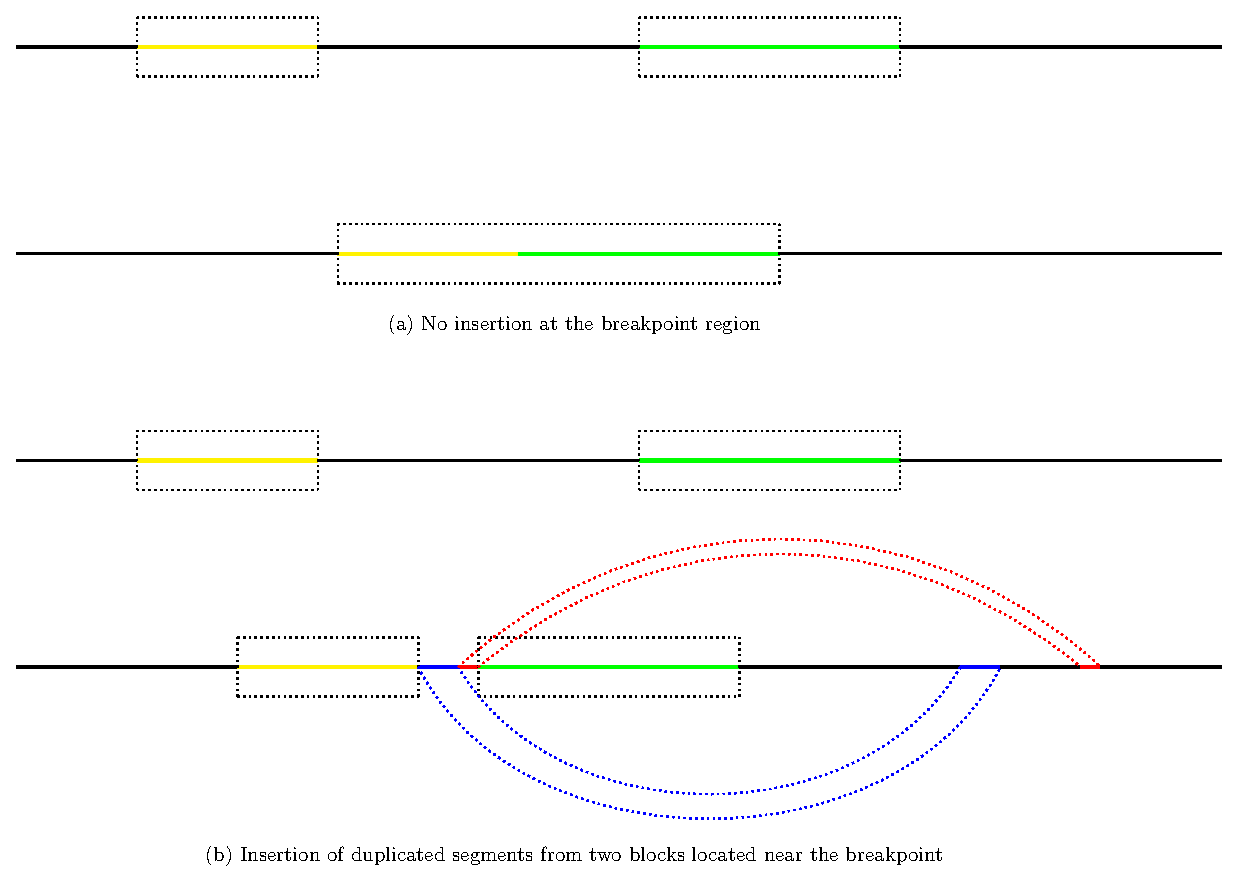
\includegraphics[width=1.0\textwidth]{breakpoint2.eps}
\caption{Examples of no insertion and complex insertions at breakpoint regions}
\label{breakpoint2}
\end{center}
\end{figure}

We hypothesize that the formation of complex breakpoint regions of rearrangements involves a replication based mechanism for the following reasons.
\begin{itemize}
\item The replication based mechanism can account for complex breakpoint regions from both the human-gibbon rearrangements~\cite{girirajan2009} 
and the observed clinical rearrangement data of genomic disorders~\cite{lee2007dna,liu2011chromosome}. 
This mechanism may expand breakpoint regions by juxtaposing and inserting distantly distributed segments.
\item The original segments are usually less than 100kb away from the duplicated segments in the breakpoint region~\cite{girirajan2009}, 
and such distances are below the long distances in the observed template-switchings (e.g., 120kb to 550kb~\cite{gu2008mechanisms}).
\item Microhomology~(2-6 bp) was observed in 50\% of the human-gibbon breakpoint regions~\cite{girirajan2009}, 
as well as many breakpoint regions from clinical data of genomic disorders~\cite{lee2007dna,liu2011chromosome}.  
\end{itemize}


We will use colored de Bruijn graphs to study the breakpoint regions of rearrangements between input genomes.  
\begin{enumerate}
\item For primate genomes, we first need to deal with the high-multiplicity mobile elements (e.g. SINE and LINE repeats). 
 The most common SINE repeats in primates are called Alu elements, each approximately 260 base pairs long. 
 The human genome contains estimated over one million Alu elements---about $11\%$ of the genome~\cite{lander2001}, 
 and about half a million LINE repeats---about $17\%$ of the genome~\cite{cordaux2009}. 
 We could mask all known the Alu elements and LINE repeats, by replacing them with random sequences of same lengths, 
 but still record their position information for later analysis, since these high-multiplicity mobile elements may contribute into the complex breakpoint regions~\cite{girirajan2009} 
 and serve as footprints at the breakpoint junctions~\cite{carvalho2011inverted}.
 \item We build a colored de Bruijn graph from the input genomes, by transforming that genomes into perfect sequencing reads of (k+1)-mer (overlapping and uniform coverage) 
 and coloring the reads of different genomes respectively. Note that this colored de Bruijn graph can only ``glue'' all perfect repeats of the same color without any gaps and mismatches. 
 We could handle imperfect repeats by the techniques in SPAdes~\cite{spades} (e.g., error corrections in reads and simplification of A-Bruijn graphs). 
 Note that we may first focus on near-perfect repeats.
 \item We find out all the candidates for breakpoints of rearrangements  and focus on candidates for complex breakpoint regions.
 A candidate is a continuous insertion sequence at the breakpoint region 
 that mainly consists of common repeat families as well as distributed segments duplicated from neighborhood of the breakpoint(see Figure~\ref{breakpoint2}(b)).
 Note that these duplicated segments are usually smaller than the rearranged segments, 
 and different parameters k should be applied to study such regions at different resolution in the colored de Bruijn graph.
\item For each candidate breakpoint region, we retrieve the sequence information from the colored de Bruijn graph, 
and check whether there are microhomology~\cite{girirajan2009,hastings2009microhomology,liu2011chromosome} at the breakpoint junctions.
\end{enumerate}

The study of complex breakpoint regions between input genomes 
may also indicate the most ``plausible'' rearrangement scenario. 
Take two genomes of 4 synteny blocks for example, say $G_1 = 1~2~3~4$ and $G_2 = ~1~$-$3~2~4$.
The breakpoint graph~\cite{bafna1993} of these two genomes consists of an alternating cycle of length 6, 
and there are two possible inversion scenarios shown in Figure~\ref{example}. 
The detailed analysis at breakpoint regions may help to find out the most ``plausible'' rearrangement scenario.
For example, in Figure~\ref{example}, if we find insertion segments from the start region of the blue block 
or the end region of the red block at the first breakpoint region (between the yellow and blue syteny blocks),
we can infer that the left scenario is more ``plausible'' than the right one, 
since it is less likely to include such insertion segments at the first breakpoint from the right scenario. Similarly, 
if we find the insertion segment from the start region of the green block 
at the second breakpoint region (between the blue and red syteny blocks), the right scenario is more likely to occur.
\begin{figure}[H]
\begin{center}
\includegraphics[width=1.0\textwidth]{example.eps}
\caption{Two possible inversion scenarios. Colored dotted curves represent several possible insertions 
at the breakpoint region, which can be used to infer the more ``plausible'' scenario of the two.}
\label{example}
\end{center}
\end{figure}


\bibliographystyle{unsrt}
\bibliography{lcbb}
\end{document}
